% ++++++++++++++++++++++++++++++++++++++++
% Don't modify this section unless you know what you're doing!
\documentclass[a4paper,12pt]{article}
\usepackage{tabularx} % extra features for tabular environment
\usepackage{amsmath}  % improve math presentation
\usepackage{graphicx} % takes care of graphic including machinery
\usepackage[margin=0.75in]{geometry} % decreases margins
\usepackage{subcaption}
\usepackage{verbatim}
\usepackage{float}
\usepackage{hyperref}
\usepackage{titling}
\hypersetup{
	colorlinks=true,       % false: boxed links; true: colored links
	linkcolor=black,        % color of internal links
	citecolor=blue,        % color of links to bibliography
	filecolor=magenta,     % color of file links
	urlcolor=blue         
}
%++++++++++++++++++++++++++++++++++++++++
\setlength{\parindent}{0pt}
\setlength\parskip{0.5em plus 0.1em minus 0.2em}
\setlength{\droptitle}{-5em}   % This is your set screw

\begin{document}
\title{DC And AC Currents Through LCR Circuits \\
\large PHY224 Fall 2021}
\author{Fredrik Dahl Bråten, Pankaj Patil}
\date{\today}
\maketitle
\begin{center}
	\section*{Abstract}
\end{center}
The aim of this experiment is  to study the behavior of different  circuit elements like 
Resistor, Capacitor and Inductor in DC and AC circuits. We observed that capacitor opposes
change in Voltage, while Inductor opposes in the current. As a result Capacitor in DC circuit is an open
circuit while Inductor in DC circuit is a short circuit. In this report we present 
these behaviors with the help of Oscilloscope measurements.

\section{Introduction}

\subsection*{A. Background Theory}
In RC circuit, the capacitance of the capacitor is given by $V_0 = \frac{Q_0}{C} \ \text{, and as we know  } I_0 = \frac{V_R}{R} \implies V_R = V_0e^{-\frac{t}{\tau}}\ \text{, where } \tau = RC$. This is also 
the fitting equation for this case. Here total Voltage $V_0$ is independent variable, and $V_R$ across the resistor is dependent variable. The capacitance (C) and the the resistance (R) are 
auxiliary parameters.

In LR circuit, we have $I_R(t) = I_0(1-e^{\frac{t}{L/R}}) \implies V_R =  V_0(1-e^{\frac{t}{L/R}})$, where $I_0  = \frac{V_0}{R}$. Our fitting equation is the same, and again total Voltage $V_0$ is our 
independent variable, and voltage across the Resistor $V_R$, is the dependent variable. $L$ and $R$ are auxiliary parameters.

In an LCR circuit, the total impedance $Z$ is defined as $Z = \sqrt{(\omega L - \frac{1}{\omega C})^2 + R^2}$. $Z$ can be found by measuring 
total Voltage $V$, compared to voltage $V_R = RI \implies Z = \frac{V}{V_R}R$.

It is clear from the fitting equation for RC circuit that we would observe exponential decay for the Voltage across the resistor, as can be seen in Figure \ref{Combined_RC_B}. And in case of LR, the relationship is reversed, and we observe exponential increase 
in voltage across the Resistor as seen in Figure \ref{Combined_LR_W}.

\subsection*{B. Materials and Methods}

In this experiment we used various circuit elements namely Resistors, Capacitors, and Inductor, in the setups provides 
in the lab manual \cite{lab-manual-ex7}. The measurements were made by connecting to the appropriate channels of Oscilloscope.

We followed the steps provided in the lab manual \cite{lab-manual-ex7} for this 
experiment. We also made adjustments based on TA's suggestion to the circuits as the 
AC circuits in the manual were applicable to old Oscilloscopes.

\section{Results}
\subsection*{A. Transient Decay (RC)}

\begin{figure}[H]
  \centerline{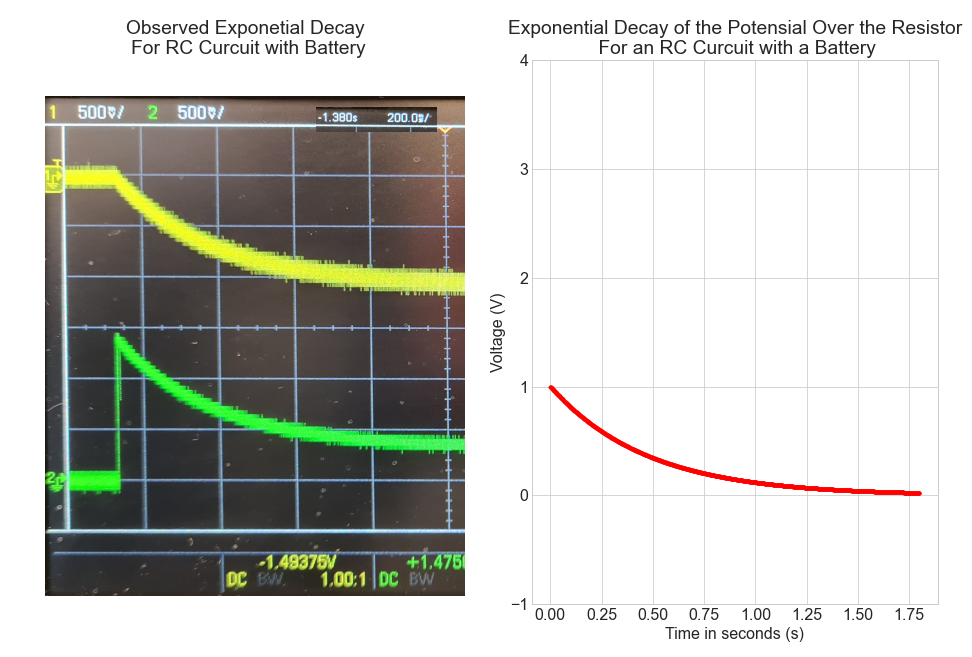
\includegraphics[width=0.75\textwidth]{../Simulated Curves/RC_B-mod.png}}
  \caption{Transient Potential Decay in RC circuit (Measurement Vs. Simulation)}
  \label{Combined_RC_B}
\end{figure}
$$\tau\ (measured) = 0.4\ s, \ \ RC = 0.47\ s$$

The observed or measured value of time constant matches closely with the theoretical value $RC$. 

\subsection*{B. DC Square Wave}

\begin{figure}[H]
  \centerline{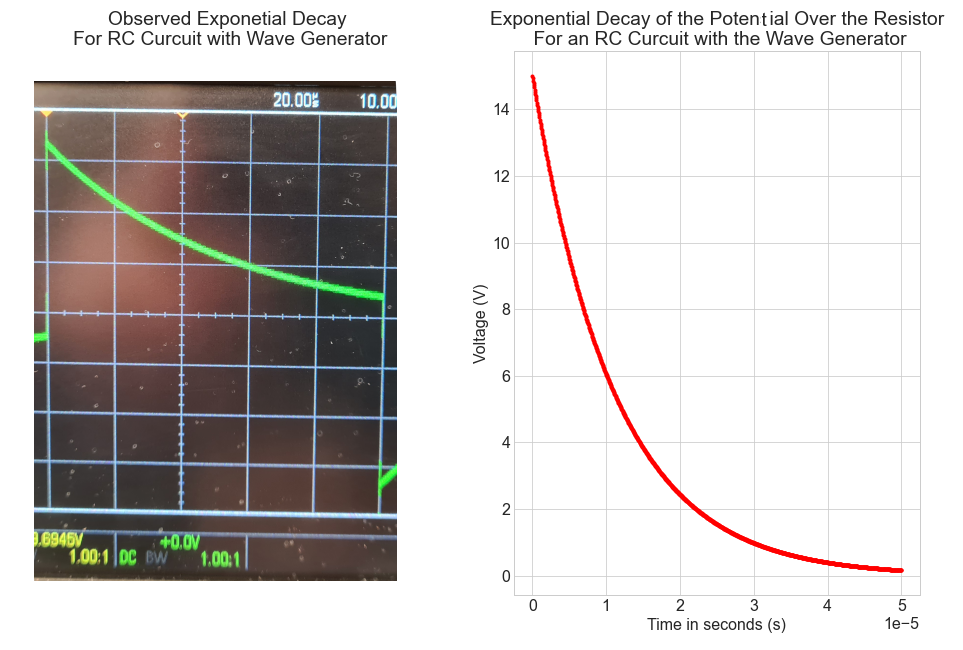
\includegraphics[width=0.75\textwidth]{../Simulated Curves/RC_W-mod.png}}
  \caption{Exponential Potential Decay in RC circuit (Measurement Vs. Simulation)}
  \label{Combined_RC_W}
\end{figure}
$$\tau\ (measured) = 8 \times 10^{-5}\ s$$
$$RC = 1.1 \times 10^{-5}\ s$$

The observed or measured value of time constant matches with the theoretical value $RC$ in order of magnitude. 

\begin{figure}[H]
  \centerline{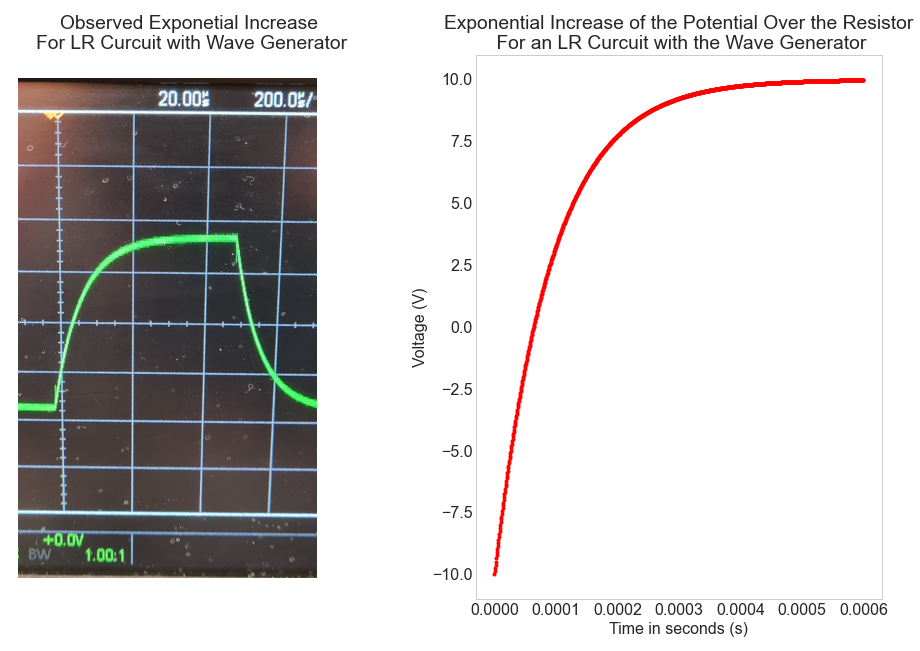
\includegraphics[width=0.9\linewidth]{../Simulated Curves/LR_W-mod.png}}
  \caption{Exponential Potential Increase in LR circuit (Measurement Vs. Simulation)}
  \label{Combined_LR_W}
\end{figure}
$$\tau\ (measured) = 5.0 \times 10^{-5}\ s$$
$$L/R = 9.2 \times 10^{-5}\ s$$

The observed or measured value of time constant matches with the theoretical value $L/R$ in order of magnitude. 

\subsection*{C. AC Sine Wave}

\begin{figure}[H]
  \centering
  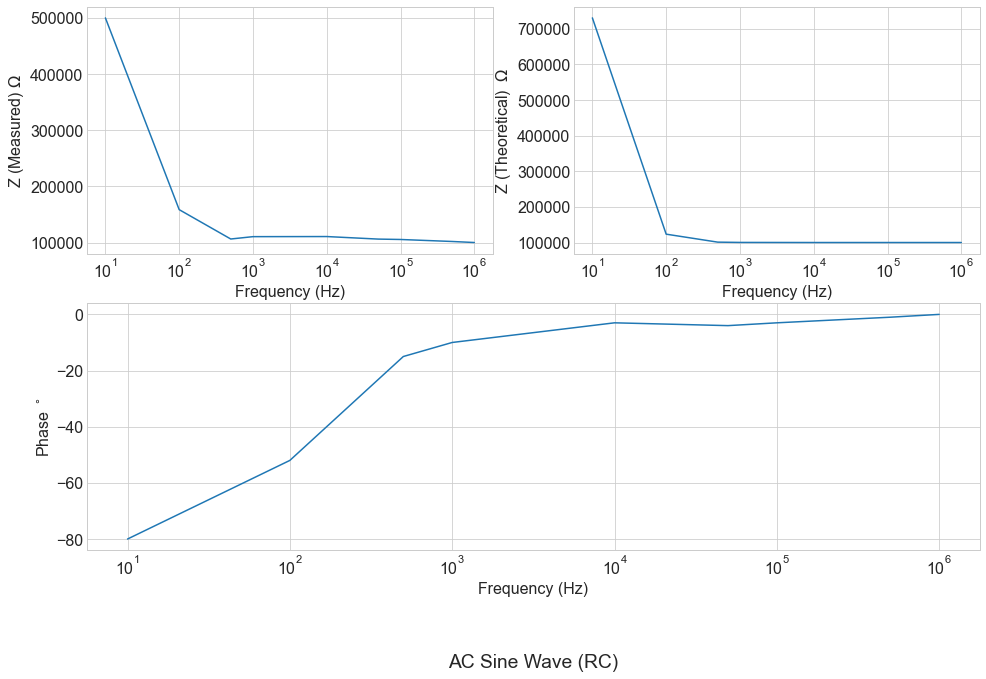
\includegraphics[width=0.8\linewidth]{../code/AC Sine Wave (RC).png}    
  \caption{AC Sine Wave (RC): Z vs Frequency and Phase vs Frequency Plots}
  \label{Combined_RC_AC}
\end{figure}

\begin{figure}[H]
  \centering
  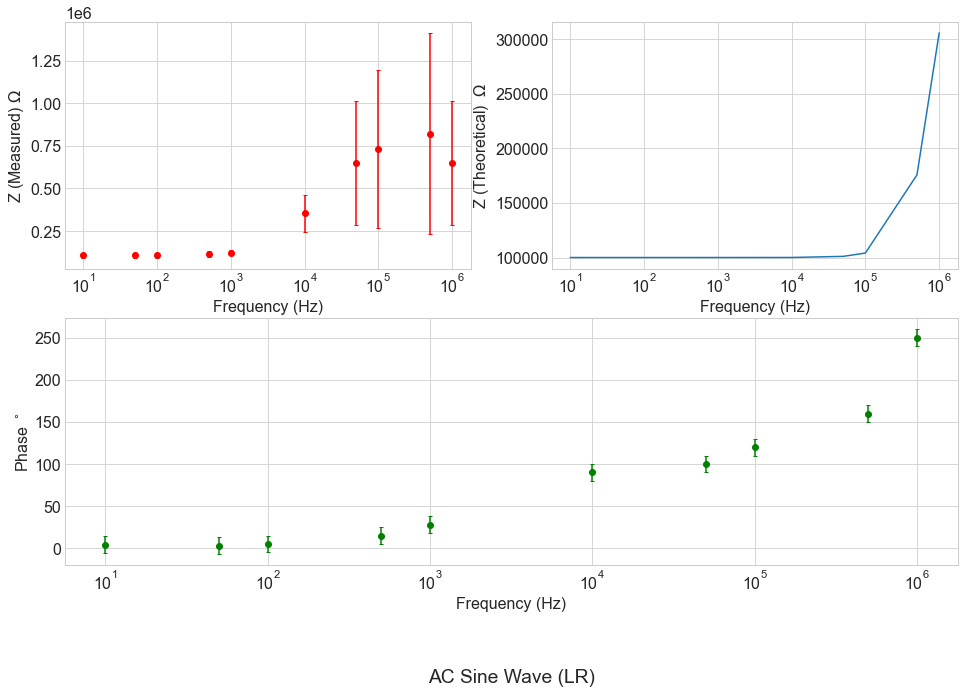
\includegraphics[width=0.8\linewidth]{../code/AC Sine Wave (LR).png}    
    \caption{AC Sine Wave (LR): Z vs Frequency and Phase vs Frequency Plots}
    \label{Combined_LR_AC}
\end{figure}

\begin{figure}[H]
  \centering
  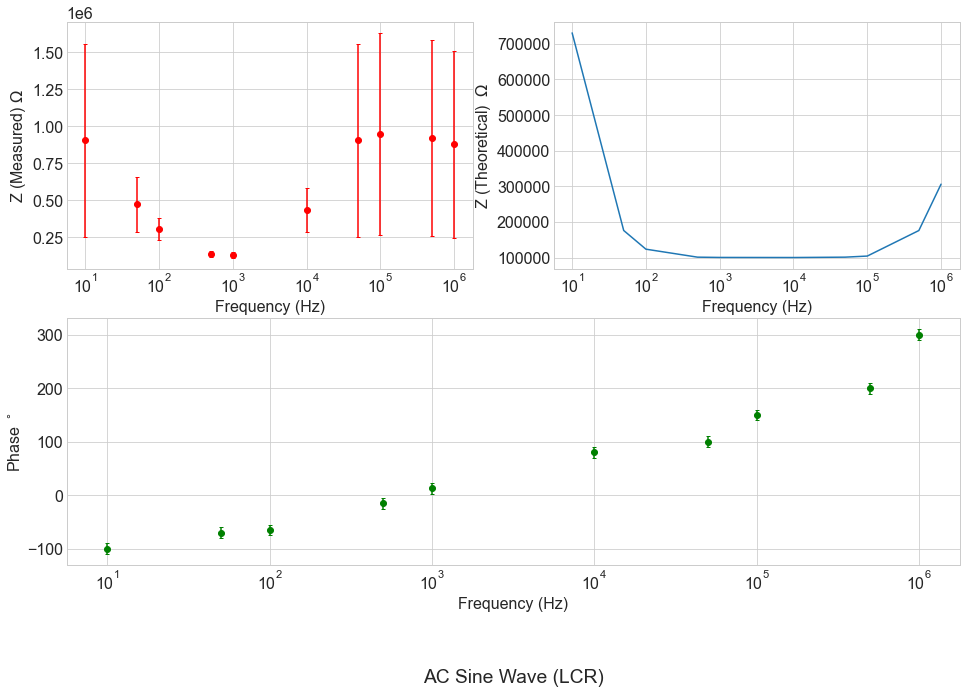
\includegraphics[width=0.8\linewidth]{../code/AC Sine Wave (LCR).png}    
    \caption{AC Sine Wave (LCR): Z vs Frequency and Phase vs Frequency Plots}
    \label{Combined_LCR_AC}
\end{figure}

\section{Uncertainty}

For the purpose of this experiment we estimated the uncertainty in $V_R$
as the thickness of the voltage line plotted on the Oscilloscope for channel 2, which 
measures the voltage across the Resistor. In case of DC circuit, with RC we observe that 
$\Delta V_R = \frac{1}{4} \times \text{Voltage Division} = .25 \times 500\ mV = 125\ mV$. 
And for DC Square Wave, it is $2\ V$. Similarly for LR Square Wave case, $\Delta V_R = 1\ V$.
Overall for the experiment we  can assume the uncertainty in the measurement of $V_R$ to be 
of the order of 1 $V$.

\section{Discussion}

In RC circuit, the accuracy of the measurement of $V_R$ in DC case is given by $\frac{|1.4/e - 1.|}{1.4/e} \times 100 = 35 \%$. 
And the precision of measurement of $V_R$ is  given by by $\frac{0.125}{0.7} \times 100 = 17 \%$. 
The accuracy value being  large can be attributed to  the  instrument.

In LR circuit, the accuracy of $V_R$ in DC case is given by $\frac{|12.64 - 10.0|}{12.64} \times 100 = 20 \%$. 
And the precision of measurement of $V_R$ is  given by by $\frac{1}{10} \times 100 = 10 \%$. 

In the LCR circuit for lower frequencies the phase difference is negative, and as the frequency is 
increased the phase gradually shifts to positive values. The resonance frequency can be estimated to be around 1 kHz. 
And as per theory $\omega_r = 1/\sqrt{LC} = 1.4$ kHz.

\pagebreak

\appendix

\section{Appendix}

\subsection{Oscilloscope Readings}

\begin{figure}[H]
  \centering
  \begin{subfigure}{.5\textwidth}
    \centering
    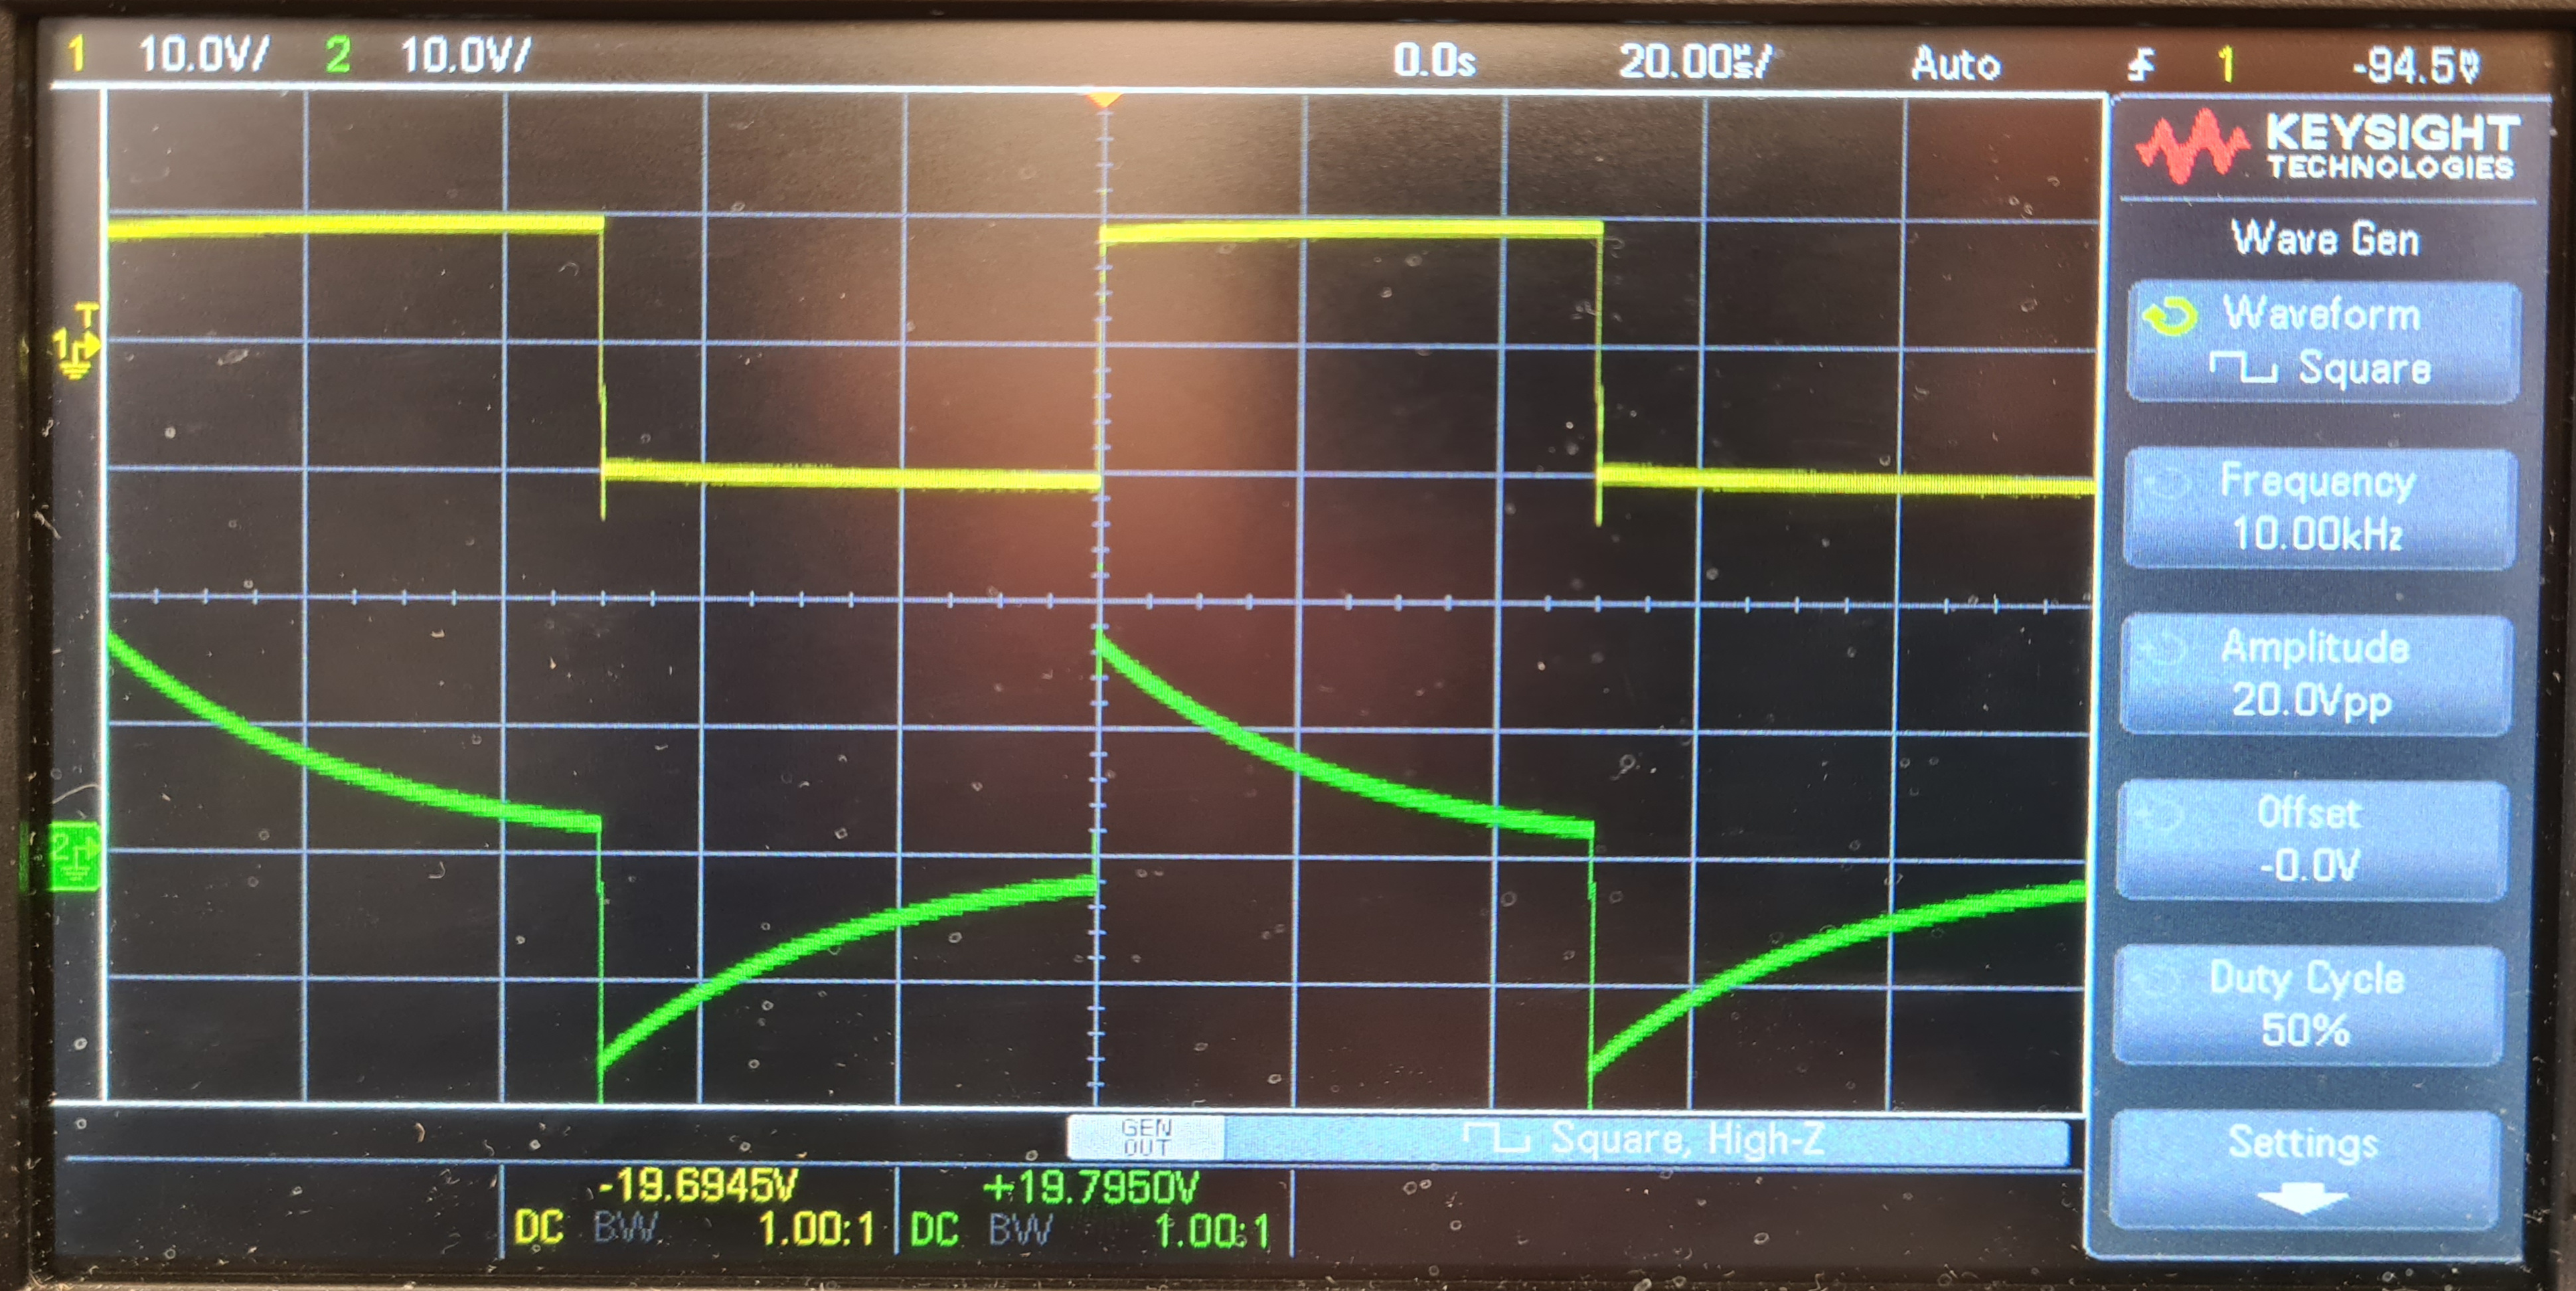
\includegraphics[width=.9\linewidth]{../data/20211116_104029-mod.jpg}
    \caption{RC Circuit with Square Wave}
  \end{subfigure}%
  \begin{subfigure}{.5\textwidth}
    \centering
    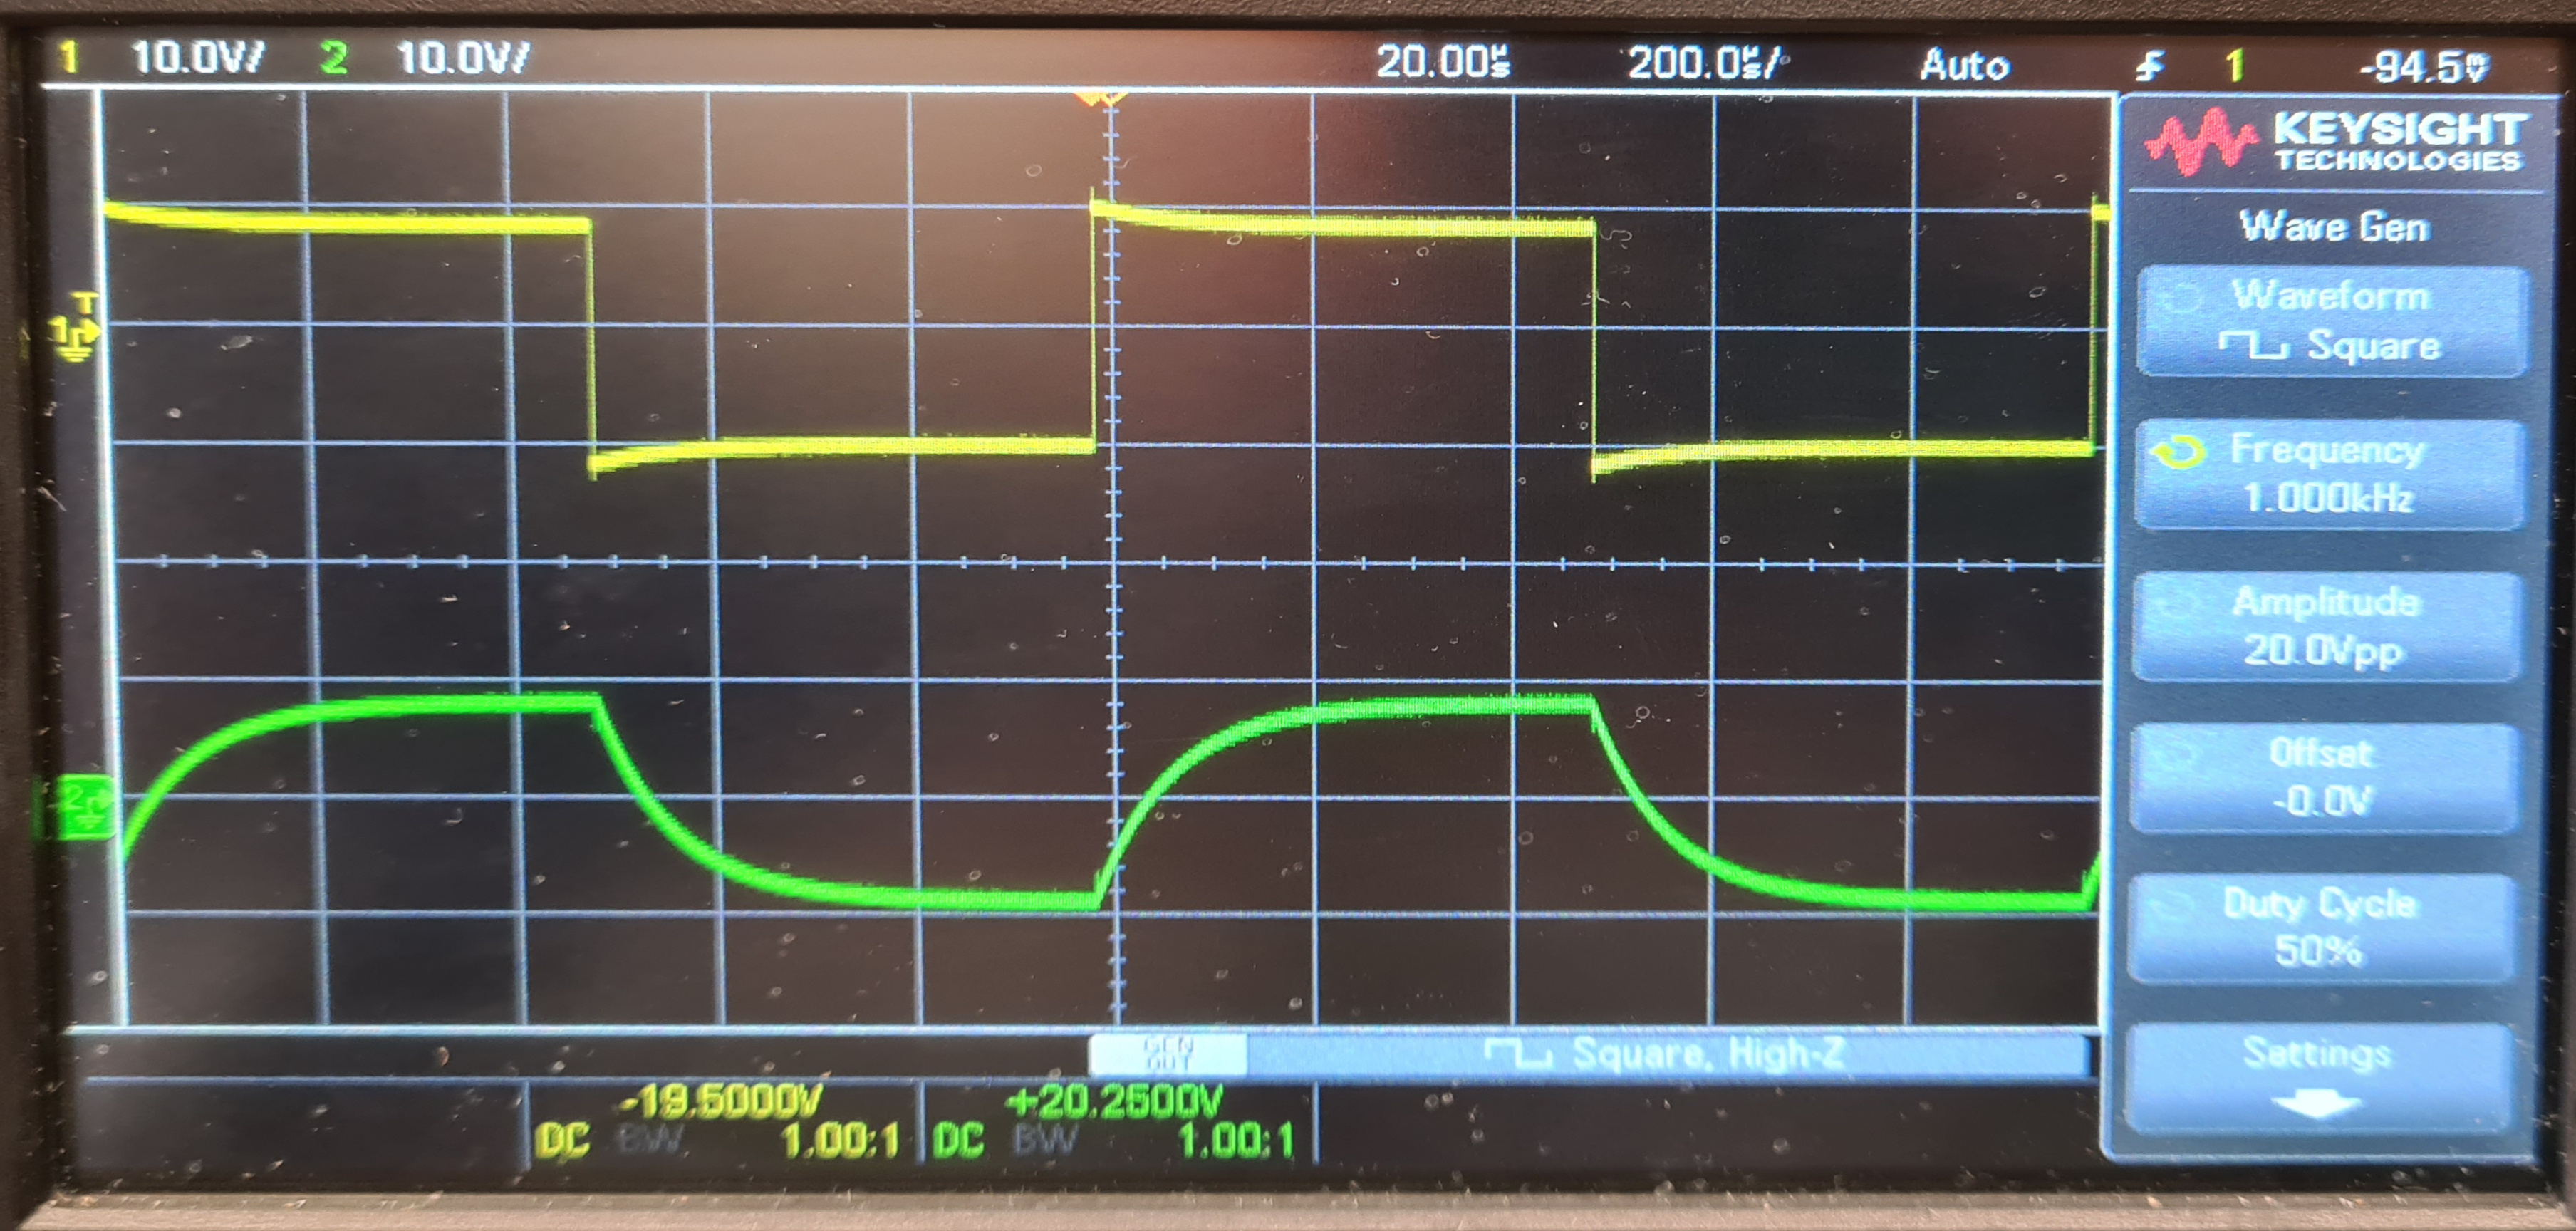
\includegraphics[width=.9\linewidth]{../data/20211116_104711-mod.jpg}
    \caption{LR Circuit with Square Wave}
  \end{subfigure}
\end{figure}

\begin{figure}[H]
  \centering
  \begin{subfigure}{.5\textwidth}
    \centering
    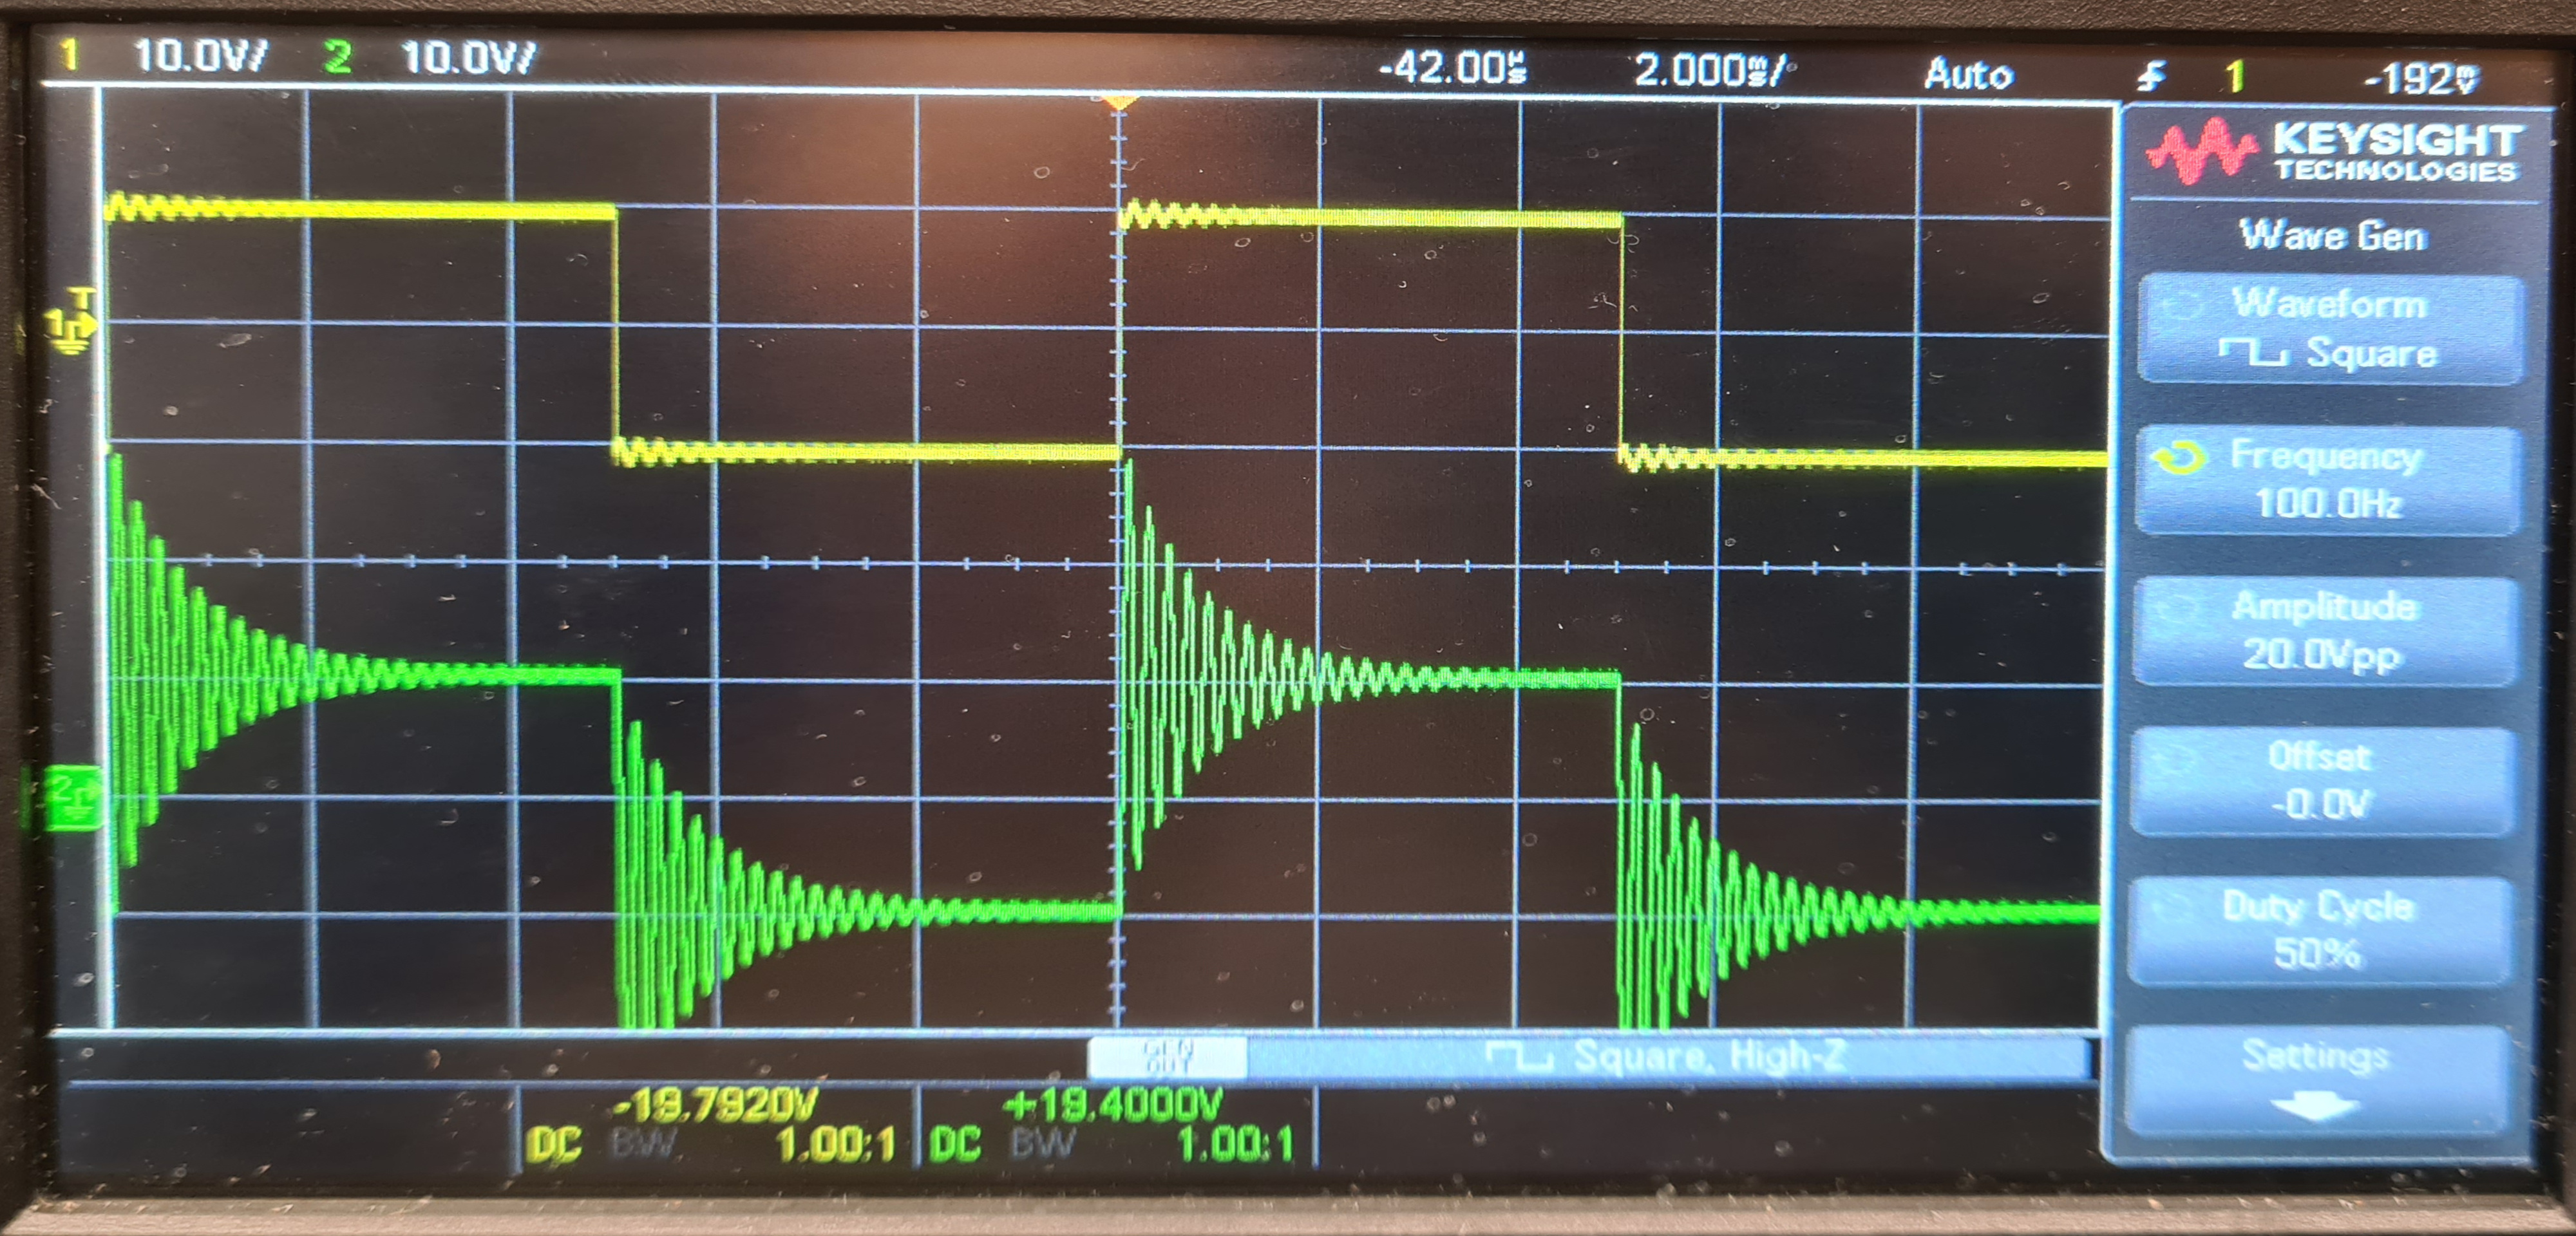
\includegraphics[width=.9\linewidth]{../data/20211116_110612-mod.jpg}
    \caption{LC Circuit with Square Wave}
  \end{subfigure}%
  \begin{subfigure}{.5\textwidth}
    \centering
    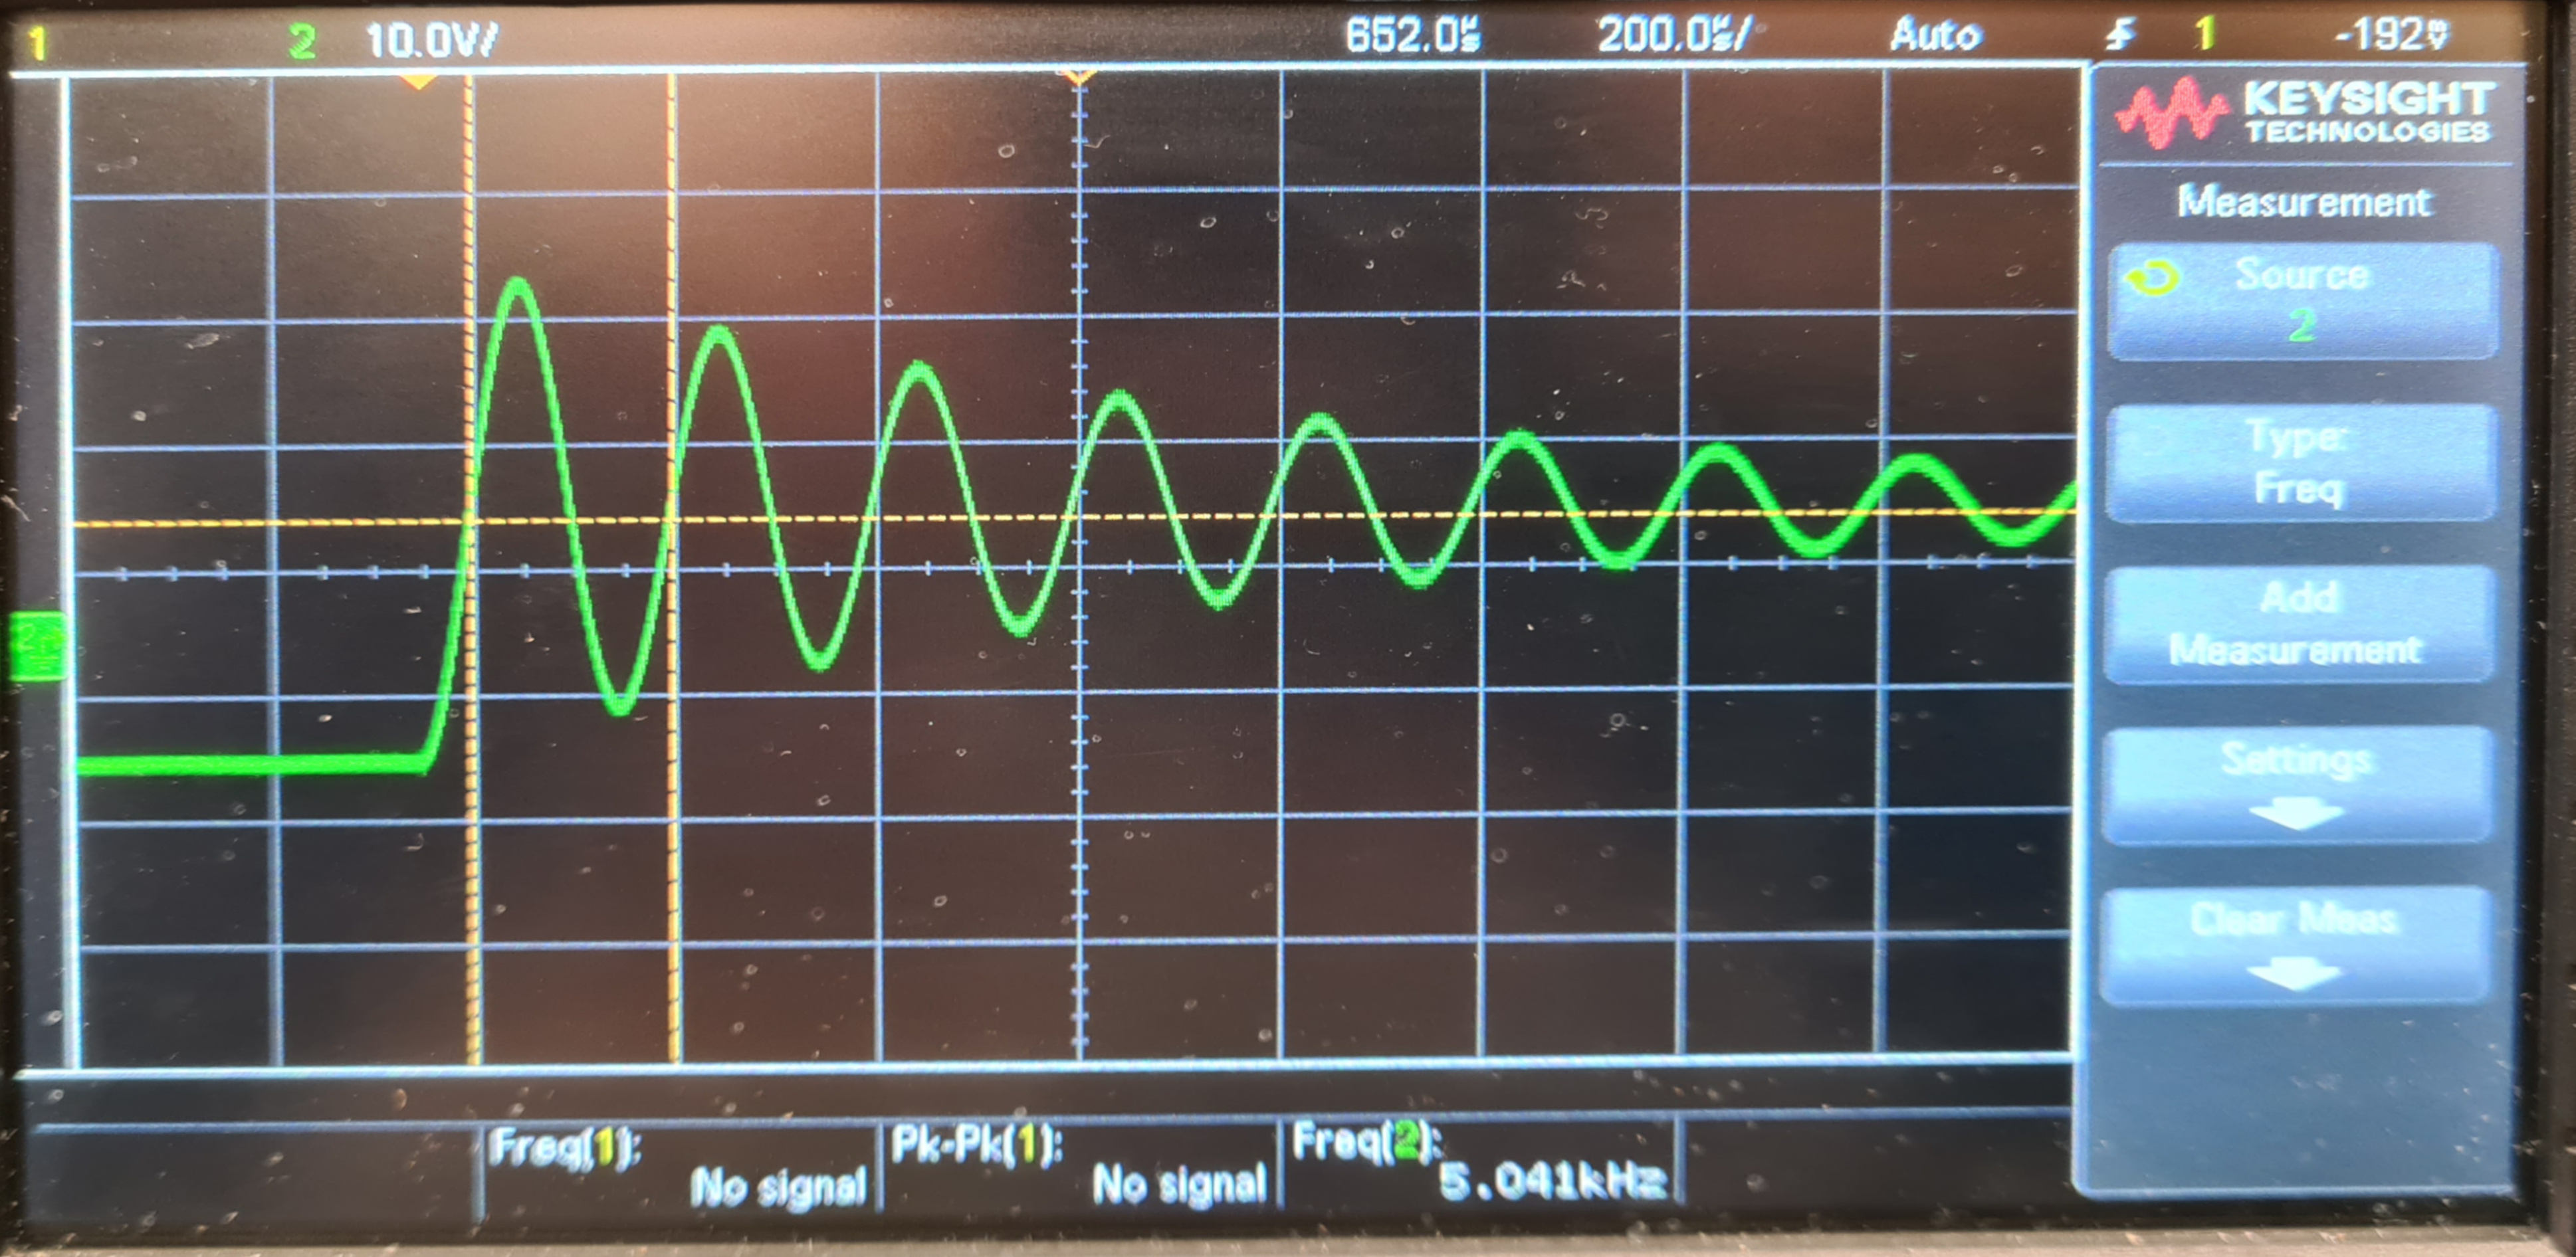
\includegraphics[width=.9\linewidth]{../data/20211116_110834-mod.jpg}
    \caption{LC Circuit with Square Wave (Zoomed In)}
  \end{subfigure}
\end{figure}

\pagebreak

\subsection{Python Code}

\subsection{Simulated Curves}

\verbatiminput{../Simulated Curves/Simulated curves.py}
\noindent\rule{\textwidth}{1pt}

\pagebreak

\subsection{Impedance and Phase Plots}

The Python code for this exercise is divided into two files. statslab.py file contains utility methods
which we will be frequently using in this course. lab\_7.py file contains the code which analyzes
the data.

\subsubsection{statslab.py}
\noindent\rule{\textwidth}{1pt}
\verbatiminput{../code/statslab.py}
\noindent\rule{\textwidth}{1pt}

\pagebreak

\subsubsection{lab\_7.py}
\noindent\rule{\textwidth}{1pt}
\verbatiminput{../code/lab_7.py}
\noindent\rule{\textwidth}{1pt}


\pagebreak

\begin{thebibliography}{99}

\bibitem{lab-manual-ex7} Currents in LCR - currents-l-c-r.pdf (\url{https://q.utoronto.ca/courses/235154/files/15436318/download?wrap=1}).

\end{thebibliography}

\end{document}
